\documentclass{article}
\usepackage{v-test-paper}
%\renewcommand{\ans}{\quad}
%\def\ansint#1{\quad}
\title{Test-Paper\\(Physics-JEE)}

\begin{document}
\maketitle

\jeeSectionA
\begin{enumerate}
\item A transverse travelling sinusoidal wave on a long stretched wire of mass per unit length $\upmu$ has frequency $\nu$ and wave speed $v$. The maximum amplitude is $A$, where $A\ll\lambda$. The wave travels towards increasing $x$. What is the energy density(energy per unit length)?
	\begin{tasks}(2)
		\task $u=\dfrac{1}{2}\upmu \omega^2A^2$\ans
		\task $u=\dfrac{1}{2}\upmu \omega^2A^2 \Delta x$
		\task $u=\dfrac{1}{2}\upmu \omega^2 A^2 v$
		\task None of these
	\end{tasks}

\item A transverse travelling sinusoidal wave on a long stretched wire of mass per unit length $\upmu$ has frequency $\nu$ and wave speed $v$. The maximum amplitude is $A$, where $A\ll\lambda$. The wave travels towards increasing $x$. What is the power transmitted along the wire?
	\begin{tasks}(2)
		\task $p=\dfrac{1}{2}\upmu \omega^2A^2$
		\task $p=\dfrac{1}{2}\upmu \omega^2A^2 \Delta x$
		\task $p=\dfrac{1}{2}\upmu \omega^2 A^2 v$\ans
		\task None of these
	\end{tasks}

\item A transverse travelling sinusoidal wave on a long stretched wire of mass per unit length $\upmu$ has frequency $\nu$ and wave speed $v$. The maximum amplitude is $A$, where $A\ll\lambda$. The wave travels towards increasing $x$. If the wave is generated by a mechanical device at $x=0$, find the transverse force $F_y(t)$ that it exerts on the wire?
	\begin{tasks}(2)
		\task $F_y(t)=\upmu v \omega A \sin(\omega t)$
		\task $F_y(t)=\upmu v \omega A \cos(\omega t)$\ans
		\task $F_y(t)=\upmu \nu \omega A \cos(\omega t)$
		\task None of these
	\end{tasks}


\item  A rope having a finite length $L$ and mass per unit length $\upmu$ hangs from a rigid support. A pulse is set up the rope by jiggling the bottom end. What is the time taken by a pulse to travel the full length of the rope?
	\begin{center}
		\begin{tikzpicture}
			\pic[rotate=-180] (ceiling) at (0, 0) {frame=2cm};
			\draw(ceiling-center)--++(0, -2.5) arc(90:-90:0.25)--++(0, -0.5);
			\tzline+[->]<0.5, 0>(0, -3)(0, 1){$v$}[mr]
		\end{tikzpicture}
	\end{center}
	\begin{tasks}(2)
		\task $2\sqrt{\dfrac{L}{g}}$\ans
		\task $2\sqrt{\dfrac{g}{L}}$	
		\task $\sqrt{\dfrac{L}{g}}$
		\task None of these
	\end{tasks}

\item  The fundamental frequency of a closed organ pipe is equal to the first overtone frequency of an open organ pipe. If length of the open pipe is $60\cm$, the length of the closed pipe will be:
	\begin{tasks}(2)
		\task $15\cm$\ans
		\task $60\cm$
		\task $45\cm$
		\task $30\cm$
	\end{tasks}

\item The velocity of sound in a gas, in which two wavelengths $4.08\m$ and $4.16\m$ produce $40$ beats in $12\s$, will be:
	\begin{tasks}(2)
		\task $282.8\mps$
		\task $175.5\mps$
		\task $353.6\mps$
		\task $707.2\mps$\ans
	\end{tasks}

\item If a wave gets refracted into a denser medium, then which of the following is true?
	\begin{tasks}(1)
		\task wavelength, speed and frequency decreases
		\task wavelength increases, speed decreases and frequency remains constant
		\task wavelength and speed decreases but frequency remains constant\ans
		\task wavelength, speed and frequency increases
	\end{tasks}

\item A tuning fork A of unknown frequency produces $5$ beats/s with a fork of known frequency $340 \Hz$. When fork A is field, the beat frequency decreases to $2$ beats/s. What is the frequency of fork A?
	\begin{tasks}(2)
		\task $338\Hz$
		\task $342\Hz$
		\task $345\Hz$
		\task $335\Hz$\ans
	\end{tasks}

\item In a resonance tube experiment when the tube is filled with water up to a height of $17.0 \cm$ from bottom, it resonates with a given tuning fork. When the water level is raised the next resonance with the same tuning fork occurs at a height of $24.5 \cm$. If the velocity of sound in air is $330 \mps$, the tuning fork frequency is :
	\begin{tasks}(2)
		\task $2200\Hz$\ans
		\task $3300\Hz$
		\task $1100\Hz$
		\task $550\Hz$
	\end{tasks}

\item Three harmonic waves having equal frequency $\nu$ and same intensity $I_0$, have phase angles $0, \dfrac{\pi}{4} \text{ and } -\dfrac{\pi}{4}$ respectively. When they are superimposed the intensity of the resultant wave is close to:
	\begin{tasks}(2)
		\task $3I_0$
		\task $I_0$
		\task $5.8I_0$\ans
		\task $0.2I_0$
	\end{tasks}

\item A tuning fork of frequency $480\Hz$ is used in an experiment for measuring speed of sound($v$) in air by resonance tube method. Resonance is observed to occur at two successive lengths of the air column, $l_1=30\cm$ and $l_2=70\cm$. Then, $v$ is equal to
	\begin{tasks}(2)
		\task $379\mps$
		\task $338\mps$
		\task $332\mps$
		\task $384\mps$\ans
	\end{tasks}

\item A small speaker delivers $2\Watt$ of audio output. At what distance from the speaker will one detect $120\text{ dB}$ intensity sound? (Take intensity of sound at threshold of hearing $I_0=10^{-12}\Watt/\m^2$)
	\begin{tasks}(2)
		\task $20\cm$
		\task $10\cm$
		\task $100\cm$
		\task $40\cm$\ans
	\end{tasks}

\item The correct figure that shows, schematically, the wave pattern produced by superposition of two waves of frequencies $9\Hz$ and $11\Hz$ is:
\def\OptionA{
	\begin{center}
		\begin{tikzpicture}
			\tzaxes(0, -1.5)(8,1.5){$t(s)$}{$y$}
			\tzticksx{pi/$1$, 2*pi/$2$}
			\tzfn{cos(deg(0.5*\x))}[0:2*pi]
			\tzfn{-cos(deg(0.5*\x))}[0:2*pi]
		\end{tikzpicture}
	\end{center}
}
\def\OptionB{
	\begin{center}
		\begin{tikzpicture}
			\tzaxes(0, -1.5)(8,1.5){$t(s)$}{$y$}
			\tzticksx{pi/$1$, 2*pi/$2$}
			\tzfn{sin(deg(\x))}[0:2*pi]
			\tzfn{-sin(deg(\x))}[0:2*pi]
		\end{tikzpicture}
	\end{center}
}
\def\OptionC{
	\begin{center}
		\begin{tikzpicture}
			\tzaxes(0, -1.5)(8,1.5){$t(s)$}{$y$}
			\tzticksx{pi/$1$, 2*pi/$2$}
			\tzfn{cos(deg(2*\x))}[0:2*pi]
			\tzfn{-cos(deg(2*\x))}[0:2*pi]
		\end{tikzpicture}
	\end{center}
}
\def\OptionD{
	\begin{center}
		\begin{tikzpicture}
			\tzaxes(0, -1.5)(8,1.5){$t(s)$}{$y$}
			\tzticksx{pi/$1$, 2*pi/$2$}
			\tzfn{cos(deg(\x))}[0:2*pi]
			\tzfn{-cos(deg(\x))}[0:2*pi]
		\end{tikzpicture}
	\end{center}
}
	\begin{tasks}
		\task \OptionA
		\task \OptionB
		\task \OptionC\ans
		\task \OptionD
	\end{tasks}







































\item 

\item 
\item 

\item 
\pagebreak










 



\end{enumerate}

\pagebreak

\jeeSectionB
\begin{enumerate}\addtocounter{enumi}{20}
\item The equation of wave is given by \[ y(x, t) = 10^{-2}\sin\left(320\pi t -\pi x + \dfrac{\pi^2}{2}\right) \] where $x$ and $y$ are in $\m$ and $t$ in $\s$. The speed of the wave is \hrulefill $\km/\h$\ansint{1152}

\item A guitar string of length $90 \cm$ vibrates with a fundamental frequency of $120 \Hz$. The length of the string producing a fundamental frequency of $180 \Hz$ will be \hrulefill $\cm$. \ansint{60}

\item The displacement equations of two interfering waves are given by
	\begin{align*}
		y_1 &= 10\sin\left(\omega t + \dfrac{\pi}{3}\right) \cm\\
		y_2 &= 5\sin\left(\omega t\right) + \sqrt{3}\cos\left(\omega t\right) \cm
	\end{align*}
	respectively. The amplitude of the resultant wave is \hrulefill $\cm$. \ansint{20}

\item The distance between two consecutive points with phase difference of $60^\circ$ in a wave of frequency $500 \Hz$ is $6.0 \m$. The velocity with which wave is travelling is \hrulefill $\km/\s$. \ansint{18}

\item Two travelling waves of equal amplitudes and equal frequencies move in opposite directions along a string. They interfere to produce a stationary wave whose equation is given by \[ y=10\cos\left(\pi x\right)\sin\left(\dfrac{2\pi}{T}t\right) \cm\] The amplitude of the particle at $x=\dfrac{4}{3} \cm$ will be \hrulefill $\cm$. \ansint{5}

\item The percentage increase in the speed of transverse waves produced in a stretched string if the tension is \linebreak increased by $4\%$, will be \hrulefill $\%$. \ansint{2} 

\item Two waves are simultaneously passing through a string and their equations are:
	\begin{align*}
		y_1 &= A_1\sin\left(kx -kvt\right) \\
		y_2 &= A_2\sin\left(kx -kvt + kx_0\right)\\
		A_1 &= 12\mm, A_2=5\mm, x_0=3.5\cm, k=6.28\cm^{-1}
	\end{align*}
	The amplitude of resulting wave will be \hrulefill $\mm$. \ansint{7}

\item Two travelling waves produces a standing wave represented by equation, \[ y(x, t) = 5\cos\left(\dfrac{\pi}{2}x\right)\sin\left(100\pi t\right)\] The node closest to the origin $x>0$ will be at $x=$ \hrulefill . \ansint{1}

\item A steel wire with mass per unit length $7.0\times 10^{-3}\kg/\m$ is under tension of $70\N$. The speed of transverse waves in the wire will be \hrulefill $\mps$. \ansint{100}
	
\item Three one-dimensional mechanical waves in an elastic medium is given as 
	\begin{align*}
		y_1 &= 3A\sin\left(\omega t - kx\right)\\
		y_2 &= A\sin\left(\omega t - kx + \pi\right)\\
		y_3 &= 2A\sin\left(\omega t + kx \right)
	\end{align*}
	are superimposed with each other. The maximum displacement amplitude of the medium particle would \linebreak be \hrulefill $A$. \ansint{4}

\end{enumerate}

\pagebreak

\begin{center}
\texttt{Answer Key}
\begin{multicols}{5}
\begin{enumerate}
\item (b)
\item (a)
\item (b)
\item (c)
\item (d)
\item (a)
\item (b)
\item (c)
\item (a)
\item (a)
\item (b)
\item (a)
\item (b)
\item (a)
\end{enumerate}
\end{multicols}
\end{center}


\end{document}
